\documentclass{article}
\usepackage[utf8]{inputenc}
\usepackage{geometry}
\usepackage[T1]{fontenc}
\usepackage{amsfonts}
\usepackage{amsmath}
\usepackage{graphicx}
\usepackage{float}
\usepackage{hyperref}
\usepackage[sorting=none]{biblatex}
\usepackage{fancyhdr}
\usepackage{multicol}
\usepackage{enumitem}
\addbibresource{ref.bib}
\setlength{\columnsep}{40pt}
\setlength{\voffset}{0.7cm}
\setlength{\headsep}{40pt}
\geometry{legalpaper, portrait, margin=2cm}


% Title page
\title{B1\\\Large{Machine Learning, Advanced Course/DD2434/mladv24}}
\author{Leonardo Lüder \\ KTH Royal Institute of Technology\\ School of Engineering Sciences in Chemistry, Biotechnology and Health}
\date{\today}

% Header and footer
\pagestyle{fancy}
\fancyhead{}
\fancyhead[L]{\textbf{Machine Learning, Advanced Course}\\\textbf{DD2434}}
\fancyhead[R]{\textbf{Leonardo Lüder}\\ luder@kth.se}
\fancyfoot{}
\begin{document}

\maketitle

% Begin page numbers
\fancyfoot[C]{\thepage}
\pagenumbering{arabic}
\begin{multicols}{2}

    \section*{Question 1.1.1:}
    Draw the DAG/PGM/Bayesian Network of the model described above.

    \textbf{Answer:}
    
    \begin{figure}[H]
        \centering
        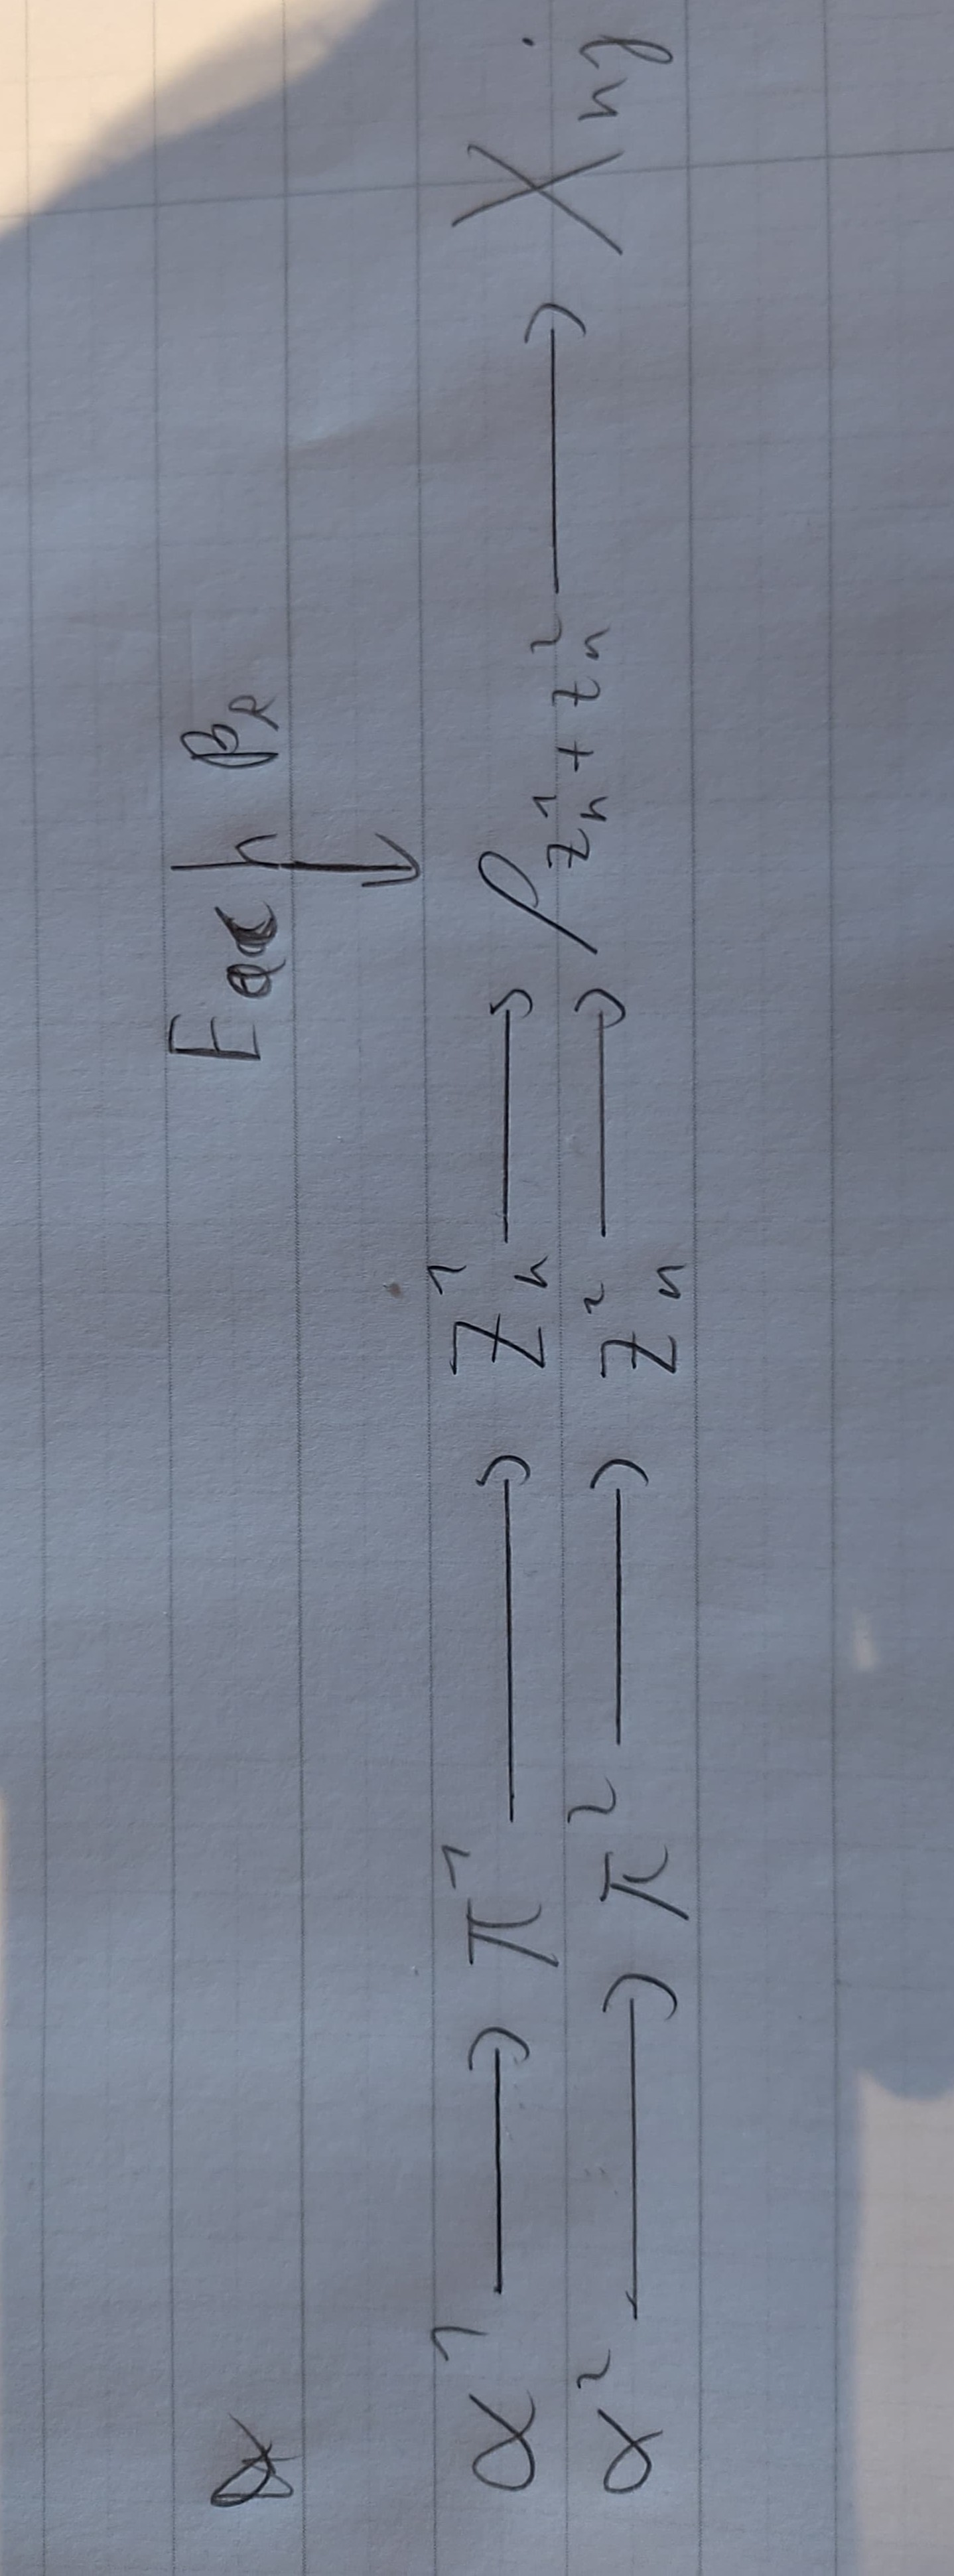
\includegraphics[width=0.4\textwidth]{figures/1/DAG.jpg}
        \caption{DAG of the model.}
    \end{figure}

    \section*{Question 1.1.2:}

    Express \( \log p(X, Z^1, Z^2, \pi^1, \pi^2, \rho | \alpha^1, \alpha^2, \beta) \) in terms of indicator functions and sums of the log of known pdfs/pmfs.  
    Do not insert the expressions for the Dirichlet distributions, e.g., write "… + \(\log p(\pi^1)\)".

    \textbf{Answer:}
    We have the joint distribution given as:
    
    \begin{multline}
    p\bigl(X, Z^1, Z^2, \pi^1, \pi^2, \rho \,\big|\,
        \alpha^1, \alpha^2, \beta\bigr) \;\\=\;
    p\bigl(\pi^1 \,\big|\,\alpha^1\bigr)\;
    p\bigl(\pi^2 \,\big|\,\alpha^2\bigr)\;
    \prod_{k} p\bigl(\rho_k \,\big|\,\beta_k\bigr) \\
    \times\; \prod_{n} \Bigl[
    p\bigl(Z^1_n \,\big|\,\pi^1\bigr)\;
    p\bigl(Z^2_n \,\big|\,\pi^2\bigr)\;
    \prod_{j} p\bigl(X_{nj} \,\big|\,\rho_{k=n}\bigr)
    \Bigr].
    \end{multline}
    

    We want \(\log p(X,Z^1,Z^2,\pi^1,\pi^2,\rho \mid \alpha^1,\alpha^2,\beta)\).

    By the model factorization:

    \[
    \begin{aligned}
    \log &p(X,Z^1,Z^2,\pi^1,\pi^2,\rho \mid \alpha^1,\alpha^2,\beta)
    \\&=
    \underbrace{\log p(\pi^1)}_{\text{Dirichlet}(\alpha^1)}
    \;+\;
    \underbrace{\log p(\pi^2)}_{\text{Dirichlet}(\alpha^2)}
    \;+\;
    \sum_{k=1}^K \underbrace{\log p(\rho_k)}_{\text{Dirichlet}(\beta_k)}
    \\
    &\quad
    +\;\sum_{n=1}^N 
    \Bigl[
    \underbrace{\log p(Z_n^1 \mid \pi^1)}_{\text{Categorical}(\pi^1)}
    \;+\;
    \underbrace{\log p(Z_n^2 \mid \pi^2)}_{\text{Categorical}(\pi^2)}
    \;+\\\;
    &\sum_{j=1}^J \underbrace{\log p\bigl(X_{nj} \mid Z_n^1+Z_n^2,\rho\bigr)}_{\text{Categorical}(\rho_{Z_n^1+Z_n^2})}
    \Bigr].
    \end{aligned}
    \]

    In indicator-function form, we write each Categorical likelihood as
    \[
    \log p(Z_n^1 = d \mid \pi^1)
    \;=\;\sum_{d=1}^{D^1}\mathbf{1}[Z_n^1 = d]\;\log \pi^1_d,
    \]  
    and similarly for \(Z_n^2\).  
    Likewise, for each observation \(X_{nj}\),  
    \[
    \log p(X_{nj}=r \mid Z_n^1+Z_n^2 = k,\, \rho_k)
    \;=\; \sum_{r=1}^{D^3} \mathbf{1}[X_{nj}=r]\;\log \rho_{k,r}.
    \]

    We combine to get:

    \[
    \begin{aligned}
    \log p(X,Z^1,Z^2,\pi^1,\pi^2,\rho \mid \alpha^1,\alpha^2,\beta)
    &\\=
    \log p(\pi^1)
    \;+\;
    \log p(\pi^2)
    \;+\;
    \sum_{k=1}^K \log p(\rho_k)
    \\
    +\;
    \sum_{n=1}^N 
    \Bigl[
    \sum_{d=1}^{D^1} \mathbf{1}[Z_n^1 = d]\;\log \pi^1_d
    \;+\;
    \sum_{e=1}^{D^2} \mathbf{1}[Z_n^2 = e]\;\log \pi^2_e
    \\
    &\quad\qquad\qquad\;\;
    +\;\sum_{j=1}^J
        \sum_{r=1}^{D^3} 
        \mathbf{1}[X_{nj}=r]\;\log \rho_{(Z_n^1 + Z_n^2),\,r}
    \Bigr].
    \end{aligned}
    \]

    \section*{Question 1.1.3:}
   
    Use the mean-field assumption:  
    \[
    q(Z^1, Z^2, \pi^1, \pi^2, \rho) = q(\pi^1)q(\pi^2)\prod_n q(Z^1_n)q(Z^2_n)\prod_k q(\rho_k)
    \]  
    and the CAVI update equation to derive the optimal variational distributions and parameters of \(q(Z^1_n)\), \(q(\pi^1)\), and \(q(\rho_k)\). 

    The mean-field assumption is given by:
    \begin{align*}
    q(Z^1, Z^2, \pi^1, \pi^2, &\rho)
    \;=\\\;
    q(\pi^1)\;q(&\pi^2)\;\prod_{n=1}^N q(Z_n^1)\;q(Z_n^2)\;\prod_{k=1}^K q(\rho_k).
    \end{align*}

    \subsection*{Update for \(q(\pi^1)\)}

    The CAVI update is given by:

    \[
    \log q(\pi^1)
    \;\;\propto\;\;
    \mathbb{E}_{q(\text{all other vars})}\bigl[\,
    \log p(X,Z^1,Z^2,\pi^1,\pi^2,\rho)
    \bigr].
    \]

    The terms involving \(\pi^1\) are:
    \begin{itemize}
        \item \(\log p(\pi^1)\) (the Dirichlet prior),
        \item \(\sum_{n=1}^N \sum_{d=1}^{D^1} \mathbf{1}[Z_n^1=d]\,\log \pi^1_d\).
    \end{itemize}

    Taking the expectation w.r.t. to all other variables replaces \(\mathbf{1}[Z_n^1=d]\) with \(q(Z_n^1=d)\).  We get:

    \[
    \log q(\pi^1)
    \;\propto\;
    \log p(\pi^1)
    \;+\;
    \sum_{n=1}^N
    \sum_{d=1}^{D^1} 
    q(Z_n^1 = d)\;\log \pi^1_d.
    \]

    \(\log p(\pi^1)\) is a Dirichlet(\(\alpha^1\)), therefore we get:

    \[
    q(\pi^1)
    \;=\;
    \mathrm{Dirichlet}
    \Bigl(
    \alpha^1_d \;+\;\sum_{n=1}^N q(Z_n^1 = d)
    \Bigr)_{d=1}^{D^1}.
    \]

    Equivalently:  
    \[
    q(\pi^1) 
    \;=\; 
    \mathrm{Dirichlet}\Bigl(\alpha^1 + m^1\Bigr),
    \quad\text{where } m^1_d = \sum_{n=1}^N q(Z_n^1 = d).
    \]

    \subsection*{Update for \(q(Z_n^1)\)}

    Again,  
    \[
    \log q(Z_n^1 = d)
    \;\;\propto\;\;
    \mathbb{E}_{q(\text{all other vars})}\bigl[\,
    \log p(X,Z^1,Z^2,\pi^1,\pi^2,\rho)
    \bigr].
    \]

    The terms involving \(Z_n^1\) are:
    \begin{itemize}
        \item \(\sum_{d=1}^{D^1} \mathbf{1}[Z_n^1=d]\;\log \pi^1_d\),
        \begin{itemize}
            \item When \(Z_n^1 = d\), contributes \(\log \pi^1_d\).
        \end{itemize}
        \item \(\sum_{j=1}^J \sum_{r=1}^{D^3} \mathbf{1}[X_{nj}=r]\;\log \rho_{(Z_n^1+Z_n^2),r}\),
        \begin{itemize}
            \item When \(Z_n^1=d\) and \(Z_n^2=e\), the index is \((d+ e)\).
            \item We must take expectation over \(Z_n^2\) as well, i.e.\ replace \(\mathbf{1}[Z_n^2 = e]\) by \(q(Z_n^2 = e)\).
        \end{itemize}
    \end{itemize}

    We get:

    
    \begin{align*}
    \log q(Z_n^1 = d)
    \propto
    \mathbb{E}_{q(\pi^1)}&\bigl[\log \pi^1_d\bigr]
    \;+\\\;
    \mathbb{E}_{q(Z_n^2),\,q(\rho)}\Bigl[
    \sum_{j=1}^J &\sum_{r=1}^{D^3} \mathbf{1}[X_{nj}=r]\;\log \rho_{(d + Z_n^2),r}
    \Bigr].
    \end{align*}
    
    \(\mathbb{E}_{q(\pi^1)}[\log \pi^1_d]\) could also be written using the digamma function, but we keep it as is. For the second term we get:

    \[
        \sum_{e=1}^{D^2} q(Z_n^2 = e)
        \sum_{j=1}^J
        \sum_{r=1}^{D^3} \mathbf{1}[X_{nj}=r]\,\mathbb{E}_{q(\rho_{d+e})}[\log \rho_{(d+e),r}].
    \]

    Exponentiating and normalizing over \(d\in\{1,\dots,D^1\}\) gives us

    \begin{align*}
        q(Z_n^1 = d)
        \;\propto\;
        \exp&\Bigl(
        \underbrace{\mathbb{E}_{q(\pi^1)}[\log \pi^1_d]}_{\text{Dirichlet posterior}}
        \;+\\\;
        \sum_{e=1}^{D^2} q(Z_n^2 = e)
            \sum_{j=1}^J &\sum_{r=1}^{D^3}
            \mathbf{1}[X_{nj}=r]\;\mathbb{E}_{q(\rho_{d+e})}[\log \rho_{(d+e),\,r}]
        \Bigr).
    \end{align*}

    \subsection*{Update for \(q(\rho_k)\)}

    The terms involving \(\rho_k\) are:

    \begin{itemize}
        \item \(\log p(\rho_k)\) (its Dirichlet prior),
        \item \(\sum_{n=1}^N \sum_{j=1}^J \sum_{r=1}^{D^3} \mathbf{1}[X_{nj}=r]\;\log \rho_{(Z_n^1+Z_n^2),r}\),
        \begin{itemize}
            \item But only those \(n\) for which \(Z_n^1 + Z_n^2 = k\).
        \end{itemize}
    \end{itemize}
    Hence,

    
    \begin{align*}
    \log q(\rho_k)
    \propto
    \log p(\rho_k)
    \;+&\\\;
    \sum_{n=1}^N
    \sum_{j=1}^J
    \sum_{r=1}^{D^3}
        \mathbf{1}[X_{nj} = r]
        \;\;&\mathbb{E}_{q(Z_n^1,\,Z_n^2)}\bigl[\mathbf{1}[Z_n^1 + Z_n^2 = k]\;\log \rho_{k,r}\bigr].
    \end{align*}
    

    \(\mathbf{1}[Z_n^1 + Z_n^2 = k]\) becomes \(\sum_{d,e}\mathbf{1}[d+e=k]\,q(Z_n^1=d)q(Z_n^2=e)\).  So

    
    \begin{align*}
    \log q(\rho_k)
    \propto
    \log p(\rho_k)
    \;+&\;
    \sum_{n=1}^N
    \sum_{j=1}^J
    \sum_{r=1}^{D^3}
        \mathbf{1}[X_{nj} = r]
        \\\Bigl[
        \sum_{d=1}^{D^1}\sum_{e=1}^{D^2}
            \mathbf{1}[d+e = k]&\,q(Z_n^1 = d)\,q(Z_n^2 = e)
        \Bigr]
        \log \rho_{k,r}.
    \end{align*}
    
    Summarize for each category \(r\in\{1,\dots,D^3\}\) as:

    \begin{align*}
    m_{k,r}
    \;=\;
    \sum_{n=1}^N
    \sum_{j=1}^J 
    \mathbf{1}[X_{nj} = r]&\\
    \sum_{d=1}^{D^1}\sum_{e=1}^{D^2}
        \mathbf{1}[d+e = k]&\,q(Z_n^1 = d)\,q(Z_n^2 = e).
    \end{align*}
    And therefore,

    \[
    \log q(\rho_k)
    \;\propto\;
    \log p(\rho_k)
    \;+\;
    \sum_{r=1}^{D^3}
    m_{k,r}\;\log \rho_{k,r}.
    \]

    \(\log p(\rho_k)\) is a \(\mathrm{Dirichlet}(\beta_k)\) prior, therefore the updated variational distribution is:

    \[
    q(\rho_k)
    \;=\;
    \mathrm{Dirichlet}\Bigl(
    \beta_k^r
    \;+\;
    m_{k,r}
    \Bigr)_{r=1}^{D^3}.
    \]

    We also note, that $q(\pi^2)$ and $q(Z_n^2)$ can be updated in a equivalently as $q(\pi^1)$ and $q(Z_n^1)$.

\end{multicols}

\clearpage
% \addcontentsline{toc}{section}{References}
% \printbibliography{}

\end{document}

